% !TeX program = pdflatex
% Companion note: one question connects Huddling, M5, the diatonic orbit, and convex energy.
% Author: Carles Marin Munoz (with AI assistance).
% Build twice with pdflatex; figure generation: python figs/huddling_figs.py from the project root.
\documentclass[11pt]{article}
\usepackage[T1]{fontenc}
\usepackage{lmodern}
\usepackage[spanish,es-noshorthands,es-tabla]{babel}
\usepackage{amsmath,amssymb,amsthm,booktabs,graphicx}
\usepackage[hidelinks]{hyperref}
\usepackage{xurl}
\usepackage[table]{xcolor}
\usepackage[margin=1in]{geometry}
\usepackage{microtype}
\usepackage{placeins}
\usepackage{tikz}
\usetikzlibrary{arrows.meta,positioning,calc}
\definecolor{ctA}{HTML}{1B6F8C}
\definecolor{ctB}{HTML}{B5530F}
\setlength{\emergencystretch}{2em}
\setlength{\textfloatsep}{14pt plus 2pt minus 3pt}
\setlength{\floatsep}{12pt plus 2pt minus 3pt}
\setlength{\intextsep}{12pt plus 2pt minus 3pt}
\renewcommand{\topfraction}{0.95}
\renewcommand{\bottomfraction}{0.85}
\renewcommand{\textfraction}{0.05}
\renewcommand{\floatpagefraction}{0.85}
\raggedbottom
\newtheorem{theorem}{Teorema}
\newtheorem{lemma}{Lema}
\newtheorem{proposition}{Proposición}
\newcommand{\lean}[1]{\texttt{#1}}
\newcommand{\Ztwelve}{\mathbb{Z}_{12}}
\newcommand{\Ahat}{\widehat A}
\newcommand{\question}[1]{\smallskip\noindent\textit{#1}\smallskip}
\newcommand{\orb}{\mathcal O_D}

\title{\bf Huddling y escalas diatónicas y pentatónicas en $\Ztwelve$:\\
máximos de Fourier y mínimos de energía convexa\\ formalizados en Lean 4}
\author{Carles Mar\'in Mu\~noz\thanks{Preparado con ayuda de herramientas de inteligencia artificial,
a partir del desarrollo previo del autor en Lean. Los resultados matemáticos son clásicos;
el autor es responsable de los enunciados, la atribución y la interpretación.
El artefacto formal y sus dependencias de confianza se describen en la Sección~\ref{sec:checked}.}\\[3pt]
\normalsize Investigador independiente\\
\normalsize \texttt{karlesmarin@gmail.com}}
\date{Octubre de 2026 \quad\textbullet\quad Versión 1.1\\[3pt]\normalsize DOI: \href{https://doi.org/10.5281/zenodo.23123219}{10.5281/zenodo.23123219}\\\href{https://github.com/karlesmarin/music-math}{github.com/karlesmarin/music-math}}

\begin{document}
\maketitle
\begin{abstract}\noindent
La colección diatónica resuelve dos problemas de optimización sobre las doce clases de altura:
maximiza el módulo del quinto coeficiente de Fourier discreto y minimiza una energía de
interacción entre todos los pares para cada potencial decreciente y discretamente convexo.
Formalizamos esta conexión en Lean~4. El recorrido comienza con el teorema de Huddling
para doce clases: en cada cardinalidad, las clases consecutivas maximizan el primer módulo
de Fourier, con igualdad exactamente en su órbita de transposición. La multiplicación por
cinco transporta este máximo a la frecuencia cinco; en cardinalidad siete, la órbita
resultante es precisamente la diatónica. Una identidad de sumación de Abel proporciona
la parte energética. Bajo convexidad y decrecimiento estrictos, las dos clases de igualdad
coinciden: para cada conjunto $A$ de siete notas,
$|\Ahat(5)|=2+\sqrt3$ si y solo si $E_V(A)=E_V(D)$.
La contribución es una formalización conectada de matemáticas clásicas en $\Ztwelve$,
con comparaciones algebraicas exactas, condiciones de igualdad explícitas y comprobaciones
ciclotómicas reproducibles e independientes. Dos certificados finitos usan evaluación
compilada de confianza (\lean{native\_decide}); la auditoría de axiomas explicita estas
dependencias. Una identidad simbólica de energía del
complemento transfiere el resultado a conjuntos pentatónicos de cinco notas sin otro censo.
La homometría, la transposición por tritono y el coeficiente de paridad conectan el
argumento con las notas anteriores.
\end{abstract}
\smallskip\noindent\textbf{Palabras clave:} lema de Huddling; escala diatónica; escala pentatónica;
conjuntos de clases de altura; transformada discreta de Fourier; máxima uniformidad;
energía convexa; Lean~4.

\section{¿Por qué aparecen dos veces las mismas siete notas?}\label{sec:hook}

Las siete teclas blancas del piano dan la colección de clases de altura
$D=\{0,2,4,5,7,9,11\}$, con $C=0$. En el reloj de doce posiciones están repartidas
alrededor del círculo. Leídas en otro orden, forman una cadena consecutiva de quintas.
Estas dos perspectivas conducen a dos propiedades extremales precisas de la misma colección.

\question{P\textsubscript{0}. ¿Por qué esta colección de siete notas maximiza un módulo
de Fourier y también minimiza una energía repulsiva entre pares?}

Los caminos históricos hacia esta pregunta fueron distintos. La nota de Lewin de 1959
sobre relaciones interválicas~\cite{Lewin} aportó una perspectiva temprana de Fourier.
El estudio de Clough y Douthett de 1991~\cite{CloughDouthett} desarrolló la máxima
uniformidad como propiedad de las escalas. Amiot recuerda un encuentro más concreto de
estas ideas: las jornadas en memoria de John Clough, celebradas en Chicago en julio de
2005, donde la tesis de Quinn contribuyó a reavivar el enfoque de Fourier de Lewin
sobre la cualidad de los acordes~\cite{Amiot2009}. El episodio recuerda que un cambio de
lenguaje matemático puede hacer visibles conexiones en materiales musicales familiares.

Douthett y Krantz relacionaron las configuraciones de máxima uniformidad con energías de
interacción y modelos unidimensionales de espines~\cite{DK}. Amiot desarrolló la
caracterización de Fourier~\cite{Amiot2007}. Esta nota sigue la conexión entre esas
perspectivas en una escala fija. Su hilo conductor es la colección diatónica: primero
como un grupo cromático consecutivo reordenado, después como maximizador de Fourier y,
finalmente, como minimizador de energía. Los enunciados en Lean explicitan el cambio
de coordenadas y la clase de igualdad.

\section{El cambio de coordenadas}\label{sec:coordinates}

Para un conjunto sin pesos $A\subseteq\Ztwelve$, usamos la DFT sin normalizar
\begin{equation}\label{eq:dft}
  \Ahat(t)=\sum_{a\in A}e^{-2\pi i at/12},\qquad
  S_t(A)=|\Ahat(t)|^2.
\end{equation}
En Lean, $A$ es un \lean{Finset (ZMod 12)} y la transformada es \lean{ZMod.dft}, de
Mathlib, aplicada a su indicadora. La función compleja \lean{Fourier.powerSpec} tiene
parte real $S_t(A)$; el enlace con el cuadrado de la norma es
\lean{Huddling.powerSpec\_re\_eq\_norm\_sq}.
La transposición $T_sA=A+s$ cambia la fase y conserva $S_t$.

\question{P\textsubscript{1}. ¿Qué coordenadas convierten un grupo cromático consecutivo
en una colección diatónica?}

Para una unidad $u\in\Ztwelve^\times$, definimos $M_uA=\{ua:a\in A\}$. Reindexar la suma finita da
\begin{equation}\label{eq:mtransform}
  \widehat{M_uA}(t)=\Ahat(ut).
\end{equation}
Este es el enunciado \lean{MTransform.Ahat\_mul}. La multiplicación por cinco es su propia
inversa módulo doce, por lo que conserva la cardinalidad e intercambia las frecuencias
uno y cinco. Cinco semitonos forman una cuarta, el sentido inverso del círculo de quintas;
esta orientación no afecta a la clase de transposición que nos ocupa.
Para $C_7=\{0,1,2,3,4,5,6\}$,
\[
 T_{11}M_5C_7=D,\qquad M_5D=T_7C_7.
\]
Ambas identidades se comprueban sobre las mismas definiciones de conjuntos usadas en los teoremas.

\begin{figure}[!htb]\centering
\begin{tikzpicture}[scale=0.87, every node/.style={font=\small}]
  \begin{scope}
    \draw[gray!60] (0,0) circle (1.65);
    \foreach \p in {0,...,11} {
      \coordinate (a\p) at ({90-30*\p}:1.65);
      \draw[fill=white,draw=gray] (a\p) circle (0.065);
      \node at ({90-30*\p}:2.00) {\p};
    }
    \foreach \p in {0,1,2,3,4,5,6} {\fill[ctA] (a\p) circle (0.085);}
    \node[align=center] at (0,-2.60) {$C_7=\{0,1,2,3,4,5,6\}$\\posiciones cromáticas consecutivas};
  \end{scope}
  \draw[-{Stealth},thick] (2.55,0.15) -- node[above,align=center] {$T_{11}\circ M_5$} (4.35,0.15);
  \begin{scope}[xshift=6.9cm]
    \draw[gray!60] (0,0) circle (1.65);
    \foreach \p in {0,...,11} {
      \coordinate (b\p) at ({90-30*\p}:1.65);
      \draw[fill=white,draw=gray] (b\p) circle (0.065);
      \node at ({90-30*\p}:2.00) {\p};
    }
    \foreach \p in {0,2,4,5,7,9,11} {\fill[ctB] (b\p) circle (0.085);}
    \draw[ctB,densely dashed] (b11)--(b4)--(b9)--(b2)--(b7)--(b0)--(b5);
    \node[align=center] at (0,-2.60) {$D=\{0,2,4,5,7,9,11\}$\\cadena consecutiva de cuartas/quintas};
  \end{scope}
\end{tikzpicture}
\caption{Las mismas siete posiciones en dos coordenadas. Los nodos rellenos indican
pertenencia; la trayectoria discontinua de la derecha suma cinco repetidamente, de $11$
a $5$. La aplicación permuta las clases de altura y los índices de Fourier, llevando
el problema del grupo consecutivo en frecuencia uno al problema diatónico en frecuencia cinco.}
\label{fig:clocks}
\end{figure}

\section{Qué aporta Huddling}\label{sec:huddling}

El lema sobre raíces de la unidad recogido por Amiot~\cite[Lema~2]{Amiot2009} establece que
las raíces consecutivas maximizan el módulo de una suma de raíces distintas. Aquí
certificamos su caso de doce clases y toda la clase de igualdad.

\begin{theorem}[Huddling en $\Ztwelve$]\label{thm:huddling}
Para cada $A\subseteq\Ztwelve$, con $k=|A|$ y $C_k=\{0,\ldots,k-1\}$,
\[
 S_1(A)\le S_1(C_k),\qquad
 S_1(A)=S_1(C_k)\ \Longleftrightarrow\ A=T_sC_k\text{ para algún }s\in\Ztwelve.
\]
La misma desigualdad y condición de igualdad se cumplen para los módulos de Fourier.
\end{theorem}

La demostración formal reduce la comparación a un orden exacto decidible. Si $i_j(A)$
cuenta los pares \emph{no ordenados} a distancia circular $j$, el enlace entre
autocorrelación y DFT de \lean{Fourier.lean} proporciona
\begin{equation}\label{eq:exact}
  2S_1(A)=P(A)+Q(A)\sqrt3,
\end{equation}
donde
\[
 P(A)=2|A|+2i_2(A)-2i_4(A)-4i_6(A),\qquad
 Q(A)=2i_1(A)-2i_5(A).
\]
El factor del tritono importa: nuestra convención para el vector interválico cuenta cada
tritono no ordenado una sola vez. \lean{MTransform.psZ} representa el miembro derecho
en $\mathbb Z[\sqrt3]$; \lean{powerSpec\_one\_re\_le\_iff} demuestra que su comparación
decidible coincide con la de las potencias reales de Fourier. La demostración no utiliza
valores trigonométricos redondeados.

El certificado finito acota los $2^{12}=4096$ conjuntos e identifica todos los casos
de igualdad. La implicación recíproca de igualdad usa simbólicamente la invariancia por
transposición. La Tabla~\ref{tab:huddling} muestra el alcance finito y las constantes exactas.
En cardinalidades cero y doce hay un único conjunto maximizador; en cada cardinalidad
intermedia hay doce, precisamente las doce rotaciones distintas de un arco consecutivo propio.

\begin{table}[!htb]\centering
\rowcolors{2}{ctA!7}{white}
\begin{tabular}{@{}cccc@{}}\toprule
\rowcolor{ctA!22}
$k$ & Conjuntos comprobados & $2S_1(C_k)$ & Maximizadores\\\midrule
$0,12$ & $1$ por cardinalidad & $0$ & $1$ por cardinalidad\\
$1,11$ & $12$ por cardinalidad & $2$ & $12$ por cardinalidad\\
$2,10$ & $66$ por cardinalidad & $4+2\sqrt3$ & $12$ por cardinalidad\\
$3,9$ & $220$ por cardinalidad & $8+4\sqrt3$ & $12$ por cardinalidad\\
$4,8$ & $495$ por cardinalidad & $12+6\sqrt3$ & $12$ por cardinalidad\\
$5,7$ & $792$ por cardinalidad & $14+8\sqrt3$ & $12$ por cardinalidad\\
$6$ & $924$ & $16+8\sqrt3$ & $12$\\\bottomrule
\end{tabular}
\caption{El censo exacto de Huddling. Las cardinalidades complementarias comparten el
máximo en frecuencia no nula, de acuerdo con la identidad de complemento de \lean{Fourier.lean}.}
\label{tab:huddling}
\end{table}

\question{P\textsubscript{2}. ¿Qué nos dice el máximo del grupo consecutivo sobre las siete teclas blancas?}

Aplicamos el Teorema~\ref{thm:huddling} a $M_5A$ y usamos la
Ecuación~\eqref{eq:mtransform}. Para $|A|=7$ obtenemos
\begin{equation}\label{eq:diatonicmax}
 S_5(A)\le S_5(D)=7+4\sqrt3,
 \qquad |\Ahat(5)|\le2+\sqrt3.
\end{equation}
La igualdad se alcanza exactamente en $\orb=\{T_sD:s\in\Ztwelve\}$.
Las inversiones de $D$ ya pertenecen a esta órbita, de modo que las descripciones por
transposición y por $T/I$ designan los mismos doce conjuntos. Por eso es apropiado
llamar \emph{diatónico} a este extremo de Fourier: la caracterización identifica la
colección salvo transposición, sin elegir una tónica ni una de sus ordenaciones modales.

\section{Por qué la energía selecciona la misma colección}\label{sec:energy}

\question{P\textsubscript{3}. ¿Podemos recuperar la clase de igualdad midiendo la separación
entre todos los pares de notas?}

Escribimos $d(a,b)=\min((a-b)\bmod12,(b-a)\bmod12)$. Para un potencial real
$V:\{1,\ldots,6\}\to\mathbb R$, la energía entre todos los pares es
\begin{equation}\label{eq:energy}
 E_V(A)=\sum_{\{a,b\}\subseteq A}V(d(a,b))
       =\sum_{j=1}^{6}i_j(A)V(j).
\end{equation}
Decimos que $V$ es admisible cuando
\begin{equation}\label{eq:admissible}
 \Delta^2V(j):=V(j)-2V(j+1)+V(j+2)\ge0\quad(1\le j\le4),
 \qquad V(6)\le V(5).
\end{equation}
Estas hipótesis implican que $V$ es no creciente: sus primeras diferencias son no
decrecientes y la última es no positiva. La admisibilidad estricta exige que las cinco
desigualdades anteriores sean estrictas. No se requiere una fórmula particular ni la
positividad de $V$.

La demostración reutiliza el argumento simbólico de \lean{AllPairsEvenness.lean}.
Para $|A|=7$, ponemos $d_j=i_{j+1}(A)-i_{j+1}(D)$, $0\le j\le5$, y
\[
 H_j=\sum_{\ell=0}^{j}(j+1-\ell)d_\ell.
\]
Ambos conjuntos tienen $\binom72=21$ pares, por lo que $\sum_{j=0}^5d_j=0$.
La doble sumación de Abel da entonces
\begin{equation}\label{eq:abel}
 E_V(A)-E_V(D)=\sum_{j=0}^{3}H_j\Delta^2V(j+1)
                      +H_4\bigl(V(5)-V(6)\bigr).
\end{equation}
Esta identidad se demuestra algebraicamente para cualquier $V$ real, con independencia
del censo. El dato finito es que $H_0,\ldots,H_4\ge0$ para cada conjunto de siete notas,
y que algún $H_j>0$ fuera de $\orb$. En $\orb$, todo el vector interválico coincide con
el de $D$. La Ecuación~\eqref{eq:abel} establece así un mínimo para cada potencial
admisible e identifica su clase de igualdad bajo las hipótesis estrictas.

\begin{theorem}[Mínimo de energía diatónico]\label{thm:energy}
Para cada $V$ admisible y cada $A\subseteq\Ztwelve$ con $|A|=7$,
$E_V(D)\le E_V(A)$. Si $V$ es estrictamente admisible, entonces
\[
 E_V(A)=E_V(D)\ \Longleftrightarrow\ A\in\orb.
\]
\end{theorem}

La estrictez es esencial en el enunciado de igualdad. Para el potencial constante $V=1$,
todos los conjuntos de siete notas tienen energía $21$, mientras que solo doce maximizan
$S_5$. Por tanto, el teorema de mínimo bajo hipótesis débiles no puede sustituir al de
unicidad estricta en la conexión siguiente.

\section{Las dos preguntas tienen una sola clase de igualdad}\label{sec:connection}

Podemos volver a P\textsubscript{0}. Huddling identifica un arco consecutivo; $M_5$ lo
convierte en la órbita diatónica; el argumento de Abel selecciona de manera independiente
esa misma órbita. La conjunción de las dos caracterizaciones da la conexión formal.

\begin{theorem}[Equivalencia entre Fourier y energía]\label{thm:connection}
Para cada $V$ estrictamente admisible y cada $A\subseteq\Ztwelve$ de siete elementos,
\[
 \boxed{\quad |\Ahat(5)|=2+\sqrt3\quad\Longleftrightarrow\quad E_V(A)=E_V(D).\quad}
\]
Ambos miembros se cumplen precisamente en las doce transposiciones de $D$.
\end{theorem}
\begin{proof}
La Ecuación~\eqref{eq:diatonicmax} identifica la clase de igualdad del miembro izquierdo
con $\orb$. El Teorema~\ref{thm:energy} identifica la del miembro derecho con $\orb$.
En Lean, el resultado es
\begin{center}\small
\lean{DiatonicExtremality.spectral\_energy\_equivalence}.
\end{center}
\end{proof}

Para el potencial concreto estrictamente admisible $V_0(j)=(7-j)^2$, el vector interválico
diatónico es $(2,5,4,3,6,1)$ y su energía es $313$. La Figura~\ref{fig:energy} muestra
todos los conjuntos de siete notas en ambas medidas. Ilustra la clase de igualdad
compartida; el teorema cuantifica sobre cada $V$ estrictamente admisible, no solo sobre
el ejemplo representado.

\begin{figure}[!htb]\centering
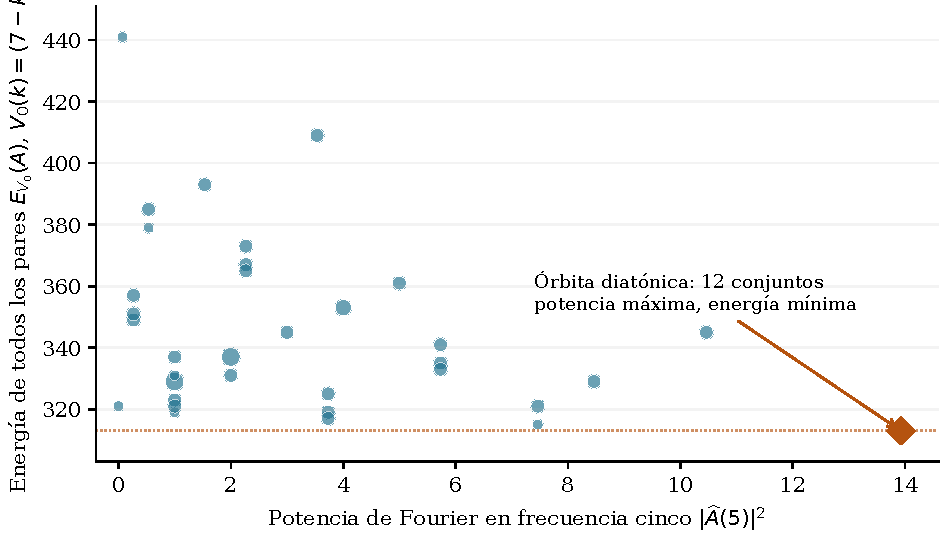
\includegraphics[width=0.94\linewidth]{figs/huddling_energy_es.pdf}
\caption{Los $792$ conjuntos de siete notas, agrupados en $34$ clases exactas de
(potencia de Fourier, energía); el área del marcador aumenta con la multiplicidad.
El rombo representa las doce transposiciones diatónicas, que alcanzan a la vez el mayor
$S_5$ y el menor $E_{V_0}$. Las coordenadas se calculan exactamente antes de convertirlas
en números para la gráfica. La coincidencia de los optimizadores no implica una
correspondencia de orden para cada par de conjuntos.}
\label{fig:energy}
\end{figure}

La nota anterior sobre la firma de Fourier por voz~\cite{Voice} usaba $a_5$ para medir
el carácter diatónico en distribuciones ponderadas por duración. El presente teorema
explica la interpretación extremal de ese nombre para conjuntos. Su dominio son las
indicadoras binarias de cardinalidad siete: los pesos de duración arbitrarios requieren
sus propias restricciones, y las observaciones empíricas sobre las voces no se deducen
de este teorema de conjuntos finitos.

\section{¿Qué ocurre con las cinco notas restantes?}\label{sec:complements}

\question{P\textsubscript{4}. ¿Heredan las teclas negras ambas propiedades extremales de las blancas?}

Sea $P=\{0,2,4,7,9\}$ la colección pentatónica anhemitónica. Las cinco teclas negras
forman $D^c=T_6P$. La complementación ya pertenece al lenguaje de Fourier de la
Nota~2~\cite{Phase}: para $t\ne0$, $\widehat{A^c}(t)=-\Ahat(t)$, de modo que los módulos
coinciden. Esta identidad y la conservación de la máxima uniformidad por complementación
son clásicas~\cite{Amiot2006}. En el lado energético debemos respetar la convención de
tritonos no ordenados. Nuestra demostración simbólica cuenta primero las notas comunes
bajo transposición:
\[
 |A^c\cap T_tA^c|+2|A|=12+|A\cap T_tA|.
\]
Por tanto, $i_j(A^c)-i_j(A)=12-2|A|$ para $1\le j\le5$, e
$i_6(A^c)-i_6(A)=6-|A|$. Multiplicar por el potencial da
\begin{equation}\label{eq:complenergy}
 E_V(A^c)-E_V(A)=(6-|A|)\left(2\sum_{j=1}^5V(j)+V(6)\right).
\end{equation}
Esta identidad no requiere convexidad. Es el caso $C_{12}$ del teorema más general de
Bushaw, Cody y Leffler sobre grafos regulares en grado por distancia~\cite[Teorema~3.5]{BCL}.
El nuevo enlace formal muestra por qué la corrección solo depende de la cardinalidad.
Para un grupo abeliano finito $G$ y un potencial par $f(x)=f(-x)$, definamos
$E_f(A)=\frac12\sum_{a,b\in A}f(b-a)$. La traslación hace constante la suma de cada fila:
$R_f=\sum_{x\in G}f(x)$. En consecuencia,
\begin{equation}\label{eq:groupcompl}
 E_f(A^c)-E_f(A)=\left(\frac{|G|}{2}-|A|\right)R_f.
\end{equation}
Los conjuntos de igual tamaño conservan por tanto su diferencia de energía al tomar
complementos; en particular, la complementación transporta los mínimos a cardinalidad
fija. En $G=\Ztwelve$, $R_f=V(0)+2\sum_{j=1}^5V(j)+V(6)$.
Nuestra energía interválica $E_V$ omite la diagonal: con $V(0)=0$, su diferencia entre
complementos coincide con la Ecuación~\eqref{eq:groupcompl}. Un conjunto de seis notas
tiene la misma energía que su complemento para cualquier potencial de distancia circular.
Son consecuencias clásicas de la simetría, enlazadas ahora en Lean con la convención
exacta de doce clases.
Para $|A|=5$, comparar con $D$ y $D^c=T_6P$ produce la identidad exacta de diferencias
\[
 E_V(A)-E_V(P)=E_V(A^c)-E_V(D).
\]
Así, el problema de cinco notas se obtiene del de siete mediante una biyección, con la
diferencia de energía conservada y el quinto coeficiente de Fourier cambiado de signo.

\begin{theorem}[Extremalidad pentatónica]\label{thm:pentatonic}
Para cada $A\subseteq\Ztwelve$ de cinco elementos, $|\Ahat(5)|\le2+\sqrt3$.
Para cada $V$ admisible, $E_V(P)\le E_V(A)$. Bajo admisibilidad estricta,
\[
 |\Ahat(5)|=2+\sqrt3\quad\Longleftrightarrow\quad
 E_V(A)=E_V(P)\quad\Longleftrightarrow\quad A=T_sP\text{ para algún }s.
\]
\end{theorem}

La demostración en Lean usa los mismos dos certificados finitos que el resultado
diatónico. El enlace por complementación es simbólico. Esto cierra también la imagen
inicial del piano: las teclas blancas y negras resuelven problemas complementarios,
y esa relación explica su aparición conjunta.

\section{Qué pueden decir ahora las notas anteriores}\label{sec:earlier}

\question{P\textsubscript{5}. ¿Puede una medida que olvida la fase identificar todavía esta escala?}

La Nota~2 estudia la homometría: igualdad de autocorrelación o, equivalentemente, de
potencia de Fourier. Nuestro enlace entre sus recuentos de intervalos ordenados y los
no ordenados de la Ecuación~\eqref{eq:energy} demuestra
\[
 A\text{ y }B\text{ homométricos}\quad\Longrightarrow\quad E_V(A)=E_V(B)
 \quad\text{para cada }V.
\]
Es una consecuencia de las descripciones clásicas equivalentes de la homometría~\cite{AS}.
Además, la homometría se conserva al tomar complementos: la identidad de autocorrelación
anterior cambia cada recuento de desplazamiento no nulo en una constante que depende solo
de la cardinalidad. Por ello, si $A,B$ son homométricos, sus complementos también lo son
y sus energías entre pares coinciden para cualquier potencial. Así se une la pregunta
sobre la fase con el enlace por complementación sin otro censo finito.
Para conjuntos generales, las energías de pares no recuperan la fase ni distinguen un
par homométrico no trivial. En el extremo diatónico, sin embargo, la unicidad espectral implica
\[
 A\text{ homométrico a }D\quad\Longleftrightarrow\quad A\in\orb.
\]
La clase de igualdad es suficientemente rígida para que, al olvidar la fase, solo quede
la ambigüedad esperada de transposición. Este corolario conecta directamente la pregunta
anterior sobre la fase con la extremalidad; no se presenta como un teorema matemático nuevo.

El mismo cambio de coordenadas conecta el tritono de la Nota~1~\cite{Tritone} con el
canal de paridad de la Nota~4~\cite{Voice}. Puesto que $5\cdot6=6\pmod{12}$,
\[
 \widehat{M_5A}(6)=\Ahat(6),\qquad M_5(T_6A)=T_6(M_5A).
\]
Así, $M_5$ intercambia las coordenadas cromática y diatónica de Fourier, conserva el
sexto coeficiente y conmuta con la transposición central por tritono. Estas identidades
no afirman que un conjunto diatónico tenga el estabilizador de 6-30, ni explican por
sí solas un efecto observado en un corpus ponderado por duración.

Por último, el espectro del Tonnetz de la Nota~3~\cite{Tonnetz} contiene $2\cos(\pi/12)$
como módulo en frecuencia cinco de una \emph{tríada} generadora. Aquí, la \emph{escala
de siete notas} extremal tiene módulo $2+\sqrt3$. La coordenada de Fourier común
conecta las medidas; sus distintas cardinalidades explican las constantes diferentes.

\section{Qué se comprueba formalmente}\label{sec:checked}

\question{P\textsubscript{6}. ¿Dónde se comprueban los enlaces de este argumento?}

\begin{figure}[!htb]\centering
\begin{tikzpicture}[box/.style={draw,rounded corners=2pt,align=center,font=\small,
  text width=5.1cm,minimum height=1.2cm},arr/.style={-{Stealth},thick},node distance=1.15cm]
  \node[box,fill=ctA!8] (h) {Huddling en $\Ztwelve$\\máximo de $S_1$\\igualdad = órbita del arco};
  \node[box,fill=ctA!8,right=1.1cm of h] (f) {$M_5$ transporta el máximo\\máximo de $S_5$\\igualdad = $\orb$};
  \node[box,fill=ctB!8,below=of h] (e) {Certificado interválico exacto\\$\sum d_j=0$, $H_j\ge0$\\fuera de la órbita: algún $H_j>0$};
  \node[box,fill=ctB!8,below=of f] (a) {Doble sumación de Abel\\$V$ estrictamente admisible\\igualdad = $\orb$};
  \node[box,text width=9.8cm,below=1.0cm of $(e)!0.5!(a)$] (c)
    {$|\Ahat(5)|=2+\sqrt3\ \Longleftrightarrow\ E_V(A)=E_V(D)$\\
    para conjuntos de siete notas y cada $V$ estrictamente admisible};
  \draw[arr] (h)--(f);
  \draw[arr] (e)--(a);
  \draw[arr] (f.south east)--++(.4,-.3)--++(0,-1.8)--(c.east);
  \draw[arr] (a)--(c);
\end{tikzpicture}
\caption{La demostración sigue dos caminos hacia la misma clase de igualdad. El de
Fourier usa Huddling y la permutación de índices; el energético usa recuentos enteros
finitos y una identidad simbólica. El teorema final une ambos caminos.}
\label{fig:proof}
\end{figure}

\begin{table}[!htb]\centering
\rowcolors{2}{ctA!7}{white}\footnotesize
\begin{tabular}{@{}p{0.47\linewidth}p{0.48\linewidth}@{}}\toprule
\rowcolor{ctA!22}
\textbf{Declaración en Lean} & \textbf{Papel en el argumento}\\\midrule
\lean{MTransform.Ahat\_mul} & Multiplicar por una unidad permuta los índices de Fourier.\\
\lean{MTransform.powerSpec\_one\_re\_le\_iff} & La comparación exacta en $\mathbb Z[\sqrt3]$ coincide con la de potencias reales.\\
\lean{Huddling.arc\_maximizes\_power}, \lean{arc\_unique} & Desigualdad de Huddling y clase de igualdad en cada cardinalidad de $\Ztwelve$.\\
\lean{Huddling.fifth\_frequency\_unique} & Transporta toda la caracterización de igualdad mediante $M_5$.\\
\lean{DiatonicExtremality.diatonic\_norm\_unique} & El máximo para siete notas es $2+\sqrt3$, exactamente en $\orb$.\\
\lean{AllPairsEvenness.abel\_bridge} & Doble sumación por partes simbólica para potenciales reales arbitrarios.\\
\lean{DiatonicExtremality.diatonic\_energy\_unique} & La misma órbita es la clase de igualdad de energía estricta.\\
\lean{DiatonicExtremality.}\newline\lean{spectral\_energy\_equivalence} & El teorema que une Fourier y energía.\\\bottomrule
\end{tabular}
\caption{Los enunciados que sostienen el relato. Los nombres sin prefijo en la fila
de Huddling pertenecen al mismo espacio de nombres.}
\label{tab:lean}
\end{table}

El archivo \lean{ExtremalityConnections.lean} añade las conexiones de las
Secciones~\ref{sec:complements}--\ref{sec:earlier}:
\begin{quote}\small
\lean{energy\_eq\_of\_homometric}, \lean{diatonic\_homometric\_iff};\\
\lean{m5\_preserves\_a6}, \lean{m5\_commutes\_tritone};\\
\lean{energy\_compl}, \lean{pentatonic\_energy\_gap};\\
\lean{pentatonic\_spectral\_energy\_equivalence}.
\end{quote}
El mismo archivo demuestra también \lean{homometric\_compl} y
\lean{energy\_compl\_eq\_of\_homometric}. El archivo separado
\lean{TranslationInvariantEnergy.lean} demuestra la forma normal para grupos finitos
\lean{energy\_compl\_card} y \lean{energy\_gap\_compl}; su especialización
\lean{PitchClassEnergy} comprueba la suma de fila, el enlace con $E_V$ y la igualdad
de energía entre hexacordos complementarios.

El desarrollo fija Lean~4.30.0-rc2 y el commit de Mathlib
\href{https://github.com/leanprover-community/mathlib4/tree/701fb6e9c3b9285968b375d19886bfc5ca134840}{\lean{701fb6e9c3b9}}
(la revisión completa está en \lean{lakefile.lean}).
Los dos censos finitos nuevos utilizan \lean{native\_decide} con aritmética exacta.
Esto añade dependencias de evaluación compilada de confianza a los axiomas fundacionales
habituales \lean{propext}, \lean{Classical.choice} y \lean{Quot.sound}; el censo completo
no se reduce dentro del núcleo. La salida explícita de \lean{\#print axioms} acompaña
la compilación. El transporte simbólico de Fourier y la identidad de Abel solo usan
los axiomas fundacionales habituales; el teorema final de extremalidad hereda además
las dos dependencias de los censos. El archivo previo \lean{AllPairsEvenness} contiene
sus propios teoremas de censo nativo, pero la interfaz nueva reutiliza su argumento
simbólico con el certificado de siete notas auditado por separado. No se emplean
\lean{sorry}, \lean{admit} ni axiomas matemáticos introducidos a mano.

Las comprobaciones independientes siguen dos caminos aritméticos: pares enteros $(P,Q)$
en \path{huddling_verify.py}, y $\mathbb Q(\zeta_{12})$ con comparaciones exactas de
reales algebraicos en \path{sage/huddling_check.py}. El segundo calcula directamente
las sumas de Fourier, con independencia de la Ecuación~\eqref{eq:exact}. Ambos verifican
los $4096$ conjuntos y los $792$ casos de siete notas en frecuencia cinco. Respaldan la
reproducibilidad; el artefacto Lean especifica el teorema.

\section{Novedad y alcance de la contribución}\label{sec:novelty}

Huddling, la permutación de índices de Fourier, la máxima uniformidad y el enfoque
energético son clásicos~\cite{Amiot2007,Amiot2009,CloughDouthett,DK}. La contribución
consiste en su formalización conectada, con las condiciones de igualdad completas para
doce clases y un teorema explícito que une los optimizadores espectrales y energéticos.
La conjunción de caracterizaciones publicadas de la clase de igualdad es un corolario,
no una caracterización nueva. El transporte de energía por complementación también
está cubierto con mayor generalidad por Bushaw, Cody y Leffler~\cite[Teoremas~2.16 y~3.5]{BCL};
las conexiones de homometría y paridad se deducen de identidades clásicas. El desarrollo
extiende las herramientas de Fourier y Abel ya presentes en este proyecto.

La revisión de antecedentes por enunciado queda recogida en
\path{literature_novelty_2026-10-03.json}. Distingue los teoremas publicados, sus
consecuencias y la cuestión de su implementación en asistentes de demostración. La
revisión dirigida establece antecedentes positivos para las matemáticas centrales;
no pretende ser un examen exhaustivo de todos los manuscritos.

Una auditoría fechada de solapamientos buscó en la instantánea de Mathlib del 3 de
octubre de 2026 ($8592$ archivos Lean) y en la instantánea examinada de Prismriver
($35$ archivos Lean), inspeccionó sus módulos relevantes de Fourier y música y realizó
búsquedas indexadas de Huddling para Lean, Coq/Rocq, Isabelle y Agda. No localizó una
formalización coincidente en esas fuentes. La auditoría registra revisiones, consultas
y cobertura en \lean{formalization\_prior\_art\_2026-10-03.json}; una búsqueda indexada
negativa no demuestra la ausencia en todos los repositorios públicos o privados.
Sí existen resultados relacionados sobre palabras de Christoffel en otro proyecto
Lean y requieren una revisión de solapamiento propia.

Todos los enunciados de Huddling de esta nota usan $\Ztwelve$; los enunciados que unen
Fourier y energía fijan las cardinalidades siete y cinco. De este censo finito no
inferimos un teorema formal para universos arbitrarios, ni identificamos los
optimizadores energético y de frecuencia cinco en todas las demás cardinalidades.
El teorema trata conjuntos sin pesos, no el orden melódico, las tónicas, la consonancia
acústica ni el origen histórico de la escala diatónica.

\section*{Coda: adónde conduce la pregunta}

La pregunta inicial tiene una respuesta exacta: las siete teclas blancas pertenecen
a una órbita seleccionada por dos funciones objetivo distintas, y $M_5$ conecta el
máximo de Fourier con un grupo consecutivo. La formalización deja una siguiente
pregunta concreta.

\question{¿Podemos sustituir el certificado finito de Huddling por una demostración
estructural en Lean para raíces de la unidad arbitrarias, conservando toda la condición de igualdad?}

El teorema matemático ya existe; la siguiente tarea consiste en hacer reutilizable su
argumento geométrico en un asistente de demostración. Con ello, el mismo cambio de
coordenadas podrá estudiarse en otros universos cíclicos. Una pregunta posterior queda
entonces formulada con precisión: ¿qué frecuencia de Fourier y qué cardinalidad
seleccionan la misma órbita que un problema dado de energía convexa? El presente
resultado de siete entre doce proporciona un caso comprobado y una interfaz común
sobre la que continuar.

\section*{Disponibilidad de datos y código}
Los archivos fuente \path{Huddling.lean}, \path{DiatonicExtremality.lean},
\path{ExtremalityConnections.lean}, \path{MTransform.lean}, \path{Fourier.lean} y
\path{AllPairsEvenness.lean} acompañan esta nota, junto con los programas de
verificación exacta y de generación de figuras, la auditoría fechada de solapamientos
y la configuración de Lake con versiones fijadas. La figura es reproducible a partir
del código; esta nota no introduce mediciones de corpus.

\FloatBarrier
\begin{thebibliography}{99}\small
\setlength{\itemsep}{3pt}
\bibitem{Lewin} D. Lewin, ``Re: Intervallic relations between two collections of notes,''
\emph{Journal of Music Theory} \textbf{3}(2) (1959), 298--301.
\href{https://doi.org/10.2307/842856}{doi:10.2307/842856}.
\bibitem{CloughDouthett} J. Clough and J. Douthett, ``Maximally even sets,''
\emph{Journal of Music Theory} \textbf{35}(1/2) (1991), 93--173.
\href{https://doi.org/10.2307/843811}{doi:10.2307/843811}.
\bibitem{Amiot2007} E. Amiot, ``David Lewin and maximally even sets,''
\emph{Journal of Mathematics and Music} \textbf{1}(3) (2007), 157--172.
\href{https://doi.org/10.1080/17459730701654990}{doi:10.1080/17459730701654990}.
\bibitem{Amiot2006} E. Amiot, ``Gammes bien r\'eparties et transform\'ee de Fourier discr\`ete,''
arXiv:math/0604210 (2006), Teoremas~2, 6 y~7.
\url{https://arxiv.org/abs/math/0604210}.
\bibitem{Amiot2009} E. Amiot, ``Discrete Fourier Transform and Bach's Good Temperament,''
\emph{Music Theory Online} \textbf{15}(2) (2009).
\url{https://mtosmt.org/issues/mto.09.15.2/mto.09.15.2.amiot.html}.
\bibitem{DK} J. Douthett and R. Krantz, ``Maximally even sets and configurations: common
threads in mathematics, physics, and music,'' \emph{Journal of Combinatorial Optimization}
\textbf{14} (2007), 385--410.
\href{https://doi.org/10.1007/s10878-006-9041-5}{doi:10.1007/s10878-006-9041-5}.
\bibitem{BCL} N. Bushaw, B. Cody, and C. Leffler, ``Sets of vertices with extremal energy,''
arXiv:2407.18785 (2024), versión~3 (2025), Teoremas~2.16 y~3.5.
\url{https://arxiv.org/abs/2407.18785}.
\bibitem{AS} E. Amiot and W. A. Sethares, ``An algebra for periodic rhythms and scales,''
manuscrito de los autores (2009), Sección~4.2.2.
\url{https://sethares.engr.wisc.edu/paperspdf/AlgofScales.pdf}.
\bibitem{Voice} C. Mar\'in Mu\~noz, ``The per-voice Fourier signature: the bass is the
spectrally purest voice,'' serie music-math (2026).
\href{https://doi.org/10.5281/zenodo.20971090}{doi:10.5281/zenodo.20971090}.
\bibitem{Phase} C. Mar\'in, ``The phase taxonomy of pitch-class set invariants,''
serie music-math, Nota~2 (2026).
\href{https://doi.org/10.5281/zenodo.20826774}{doi:10.5281/zenodo.20826774}.
\bibitem{Tritone} C. Mar\'in, ``A tritone-centered self-duality: the set class 6-30 and its
order-12 neo-Riemannian dual,'' serie music-math, Nota~1 (2026).
\href{https://doi.org/10.5281/zenodo.20820962}{doi:10.5281/zenodo.20820962}.
\bibitem{Tonnetz} C. Mar\'in, ``The Tonnetz spectrum is the generating triad's Fourier balance
profile,'' serie music-math, Nota~3 (2026).
\href{https://doi.org/10.5281/zenodo.20862822}{doi:10.5281/zenodo.20862822}.
\bibitem{Mathlib} The Mathlib Community, \emph{Mathlib4}, con el desarrollo de \lean{ZMod.dft}
por D. Loeffler. \url{https://github.com/leanprover-community/mathlib4}.
\bibitem{Prismriver} L. Aniva and C. Wang, \emph{Prismriver: Formalization of Music Theory
and Algorithmic Composition in Lean 4}, arXiv:2606.19936 (2026).
\url{https://github.com/lenianiva/Prismriver}.
\end{thebibliography}
\end{document}
